\documentclass[serif,mathserif]{beamer}
\usepackage{etex}
\usepackage{amsmath, amsfonts, epsfig, xspace}
\usepackage{algorithm,algorithmic}
\usepackage{pstricks,pst-node}
\usepackage{multimedia}
\usepackage[normal,tight,center]{subfigure}
\setlength{\subfigcapskip}{-.5em}
\usepackage{beamerthemesplit}
\usetheme{lankton-keynote}
\usepackage{color}
\usepackage{graphicx,color}
% remove caption of figure
\usepackage[labelformat=empty]{caption}

\usepackage[none]{hyphenat} % hyphenation is ugly in slides
\usepackage{parskip}

\usepackage{relsize} % \smaller to change size

\usepackage{tikz}
\usetikzlibrary{calc}

\usetikzlibrary{arrows}

\newcommand{\TikzDraw}[2][]{
  \begin{tikzpicture}[overlay, remember picture, shift={(current page.center)}, #1]
    #2
  \end{tikzpicture}
}

\newcommand{\gridlines}{
  \TikzDraw{
    \draw[help lines,xstep=.2,ystep=.2,red!20] (current page.south west) grid (current page.north east);
    \draw[help lines,xstep=1,ystep=1,red] (current page.south west) grid (current page.north east);
    \foreach \x in {-15,-14,...,15} {
      \node [anchor=north, red] at (\x,0) {\tiny \x};
      \node [anchor=east,red] at (0,\x) {\tiny \x};
    }
  }
}

\newcommand{\DrawOnImg}[3][]
{
  \begin{tikzpicture}
    \node[anchor=south west,inner sep=0] (image) at (0,0){
      #2
    };
    \begin{scope}[x={(image.south east)},y={(image.north west)}]
      \ifthenelse{\equal{#1}{grid}}
                 {\draw[color=blue, style=dashed] (0,0) grid[xstep=.1, ystep=.1] (1.0001,1.0001);}
                 {}
                 #3
    \end{scope}
  \end{tikzpicture}
}


\author[Jiong Chen]{Jiong Chen}

\title[\hspace{2em}\insertframenumber/\inserttotalframenumber]{Stable Constrained Dynamics}

\date{October 28, 2015} %leave out for today's date to be insterted

% \institute{Zhejiang University}

\newcommand{\BOLD}[1]{\mathbf{#1}}
\newcommand{\PDIF}[2]{\frac{\partial #1}{\partial #2}}

\definecolor{DARK}{RGB}{45, 33, 73}
\definecolor{LIGHT}{RGB}{119, 52, 106}
\definecolor{TEXTLIGHT}{RGB}{213, 207, 229}
\definecolor{TEXTDARK}{RGB}{66, 66, 66}
\definecolor{BULLET}{RGB}{179, 17, 102}
\definecolor{EM}{RGB}{179,17,102}

\begin{document}

\maketitle

\begin{frame}
 \frametitle{Background and Motivation}
 \begin{itemize}
  \item Two main approaches to simulate deformable bodies
    \begin{itemize}
     \item \color{red}Elasticity, for soft to moderately stiff objects
     \item \color{green}Constraints, for objects with high stiffness
    \end{itemize}
  \item Limitations of two approaches
    \begin{itemize}
      \item \color{red} Elasticity: numerically hard as stiffness increases
      \item \color{green} Constraints: instabilities in the nullspace directions
    \end{itemize}
  \item Missing piece for \textbf{\color{orange}efficiently} and \textbf{\color{orange}stablely} to simulate stiff objects?
  \pause
  \TikzDraw {
    \node [fill=DARK!50, draw=black!50, rounded corners=3mm, text opacity=1, fill opacity=0.7] at (-0.1, -3.0) {\LARGE\color{yellow}{Geometric Stiffness}};
  }
 \end{itemize}
\end{frame}

\begin{frame}
 \frametitle{Introduction to Time Integration}
 \begin{itemize}
  \item Explicit Euler
    \begin{eqnarray*}
     \BOLD{v}_+ &=& \BOLD{v} + h\BOLD{a} \\
     \BOLD{x}_+ &=& \BOLD{x} + h\BOLD{v}
    \end{eqnarray*}
  \item Symplectic Euler
   \begin{eqnarray*}
     \BOLD{v}_+ &=& \BOLD{v} + h\BOLD{a} \\
     \BOLD{x}_+ &=& \BOLD{x} + h\BOLD{v}_+
    \end{eqnarray*}
  \item Implicit Euler
    \begin{eqnarray*}
     \BOLD{v}_+ &=& \BOLD{v} + h\BOLD{a}_+ \\
     \BOLD{x}_+ &=& \BOLD{x} + h\BOLD{v}_+
    \end{eqnarray*}
 \end{itemize}
 \pause
 \TikzDraw {
    \node [fill=DARK!50, draw=black!50, rounded corners=3mm, text opacity=1, fill opacity=0.7] at (0.3, -2.8) {\huge \color{yellow}$(\BOLD{M}-h^2\BOLD{K})\BOLD{v}_+=\BOLD{p}+h\BOLD{f}$};
    \pause
    \draw[red, very thick] (-3.4,-3.4) -- (-3.4,-2.2) -- (0.2,-2.2) -- (0.2,-3.4) -- (-3.4,-3.4);
    \node at (-1.6, -3.7) {\color{green!50} augmented inertia};
    \draw[red, very thick] (1.8, -2.2) -- (1.8, -3.4) -- (2.4, -3.4) -- (2.4, -2.2) -- (1.8, -2.2);
    \node at (2.1, -1.8) { \color{green!50} current momentum};
    \draw[red, very thick] (3.2, -2.2) -- (3.2, -3.4) -- (4, -3.4) -- (4, -2.2) -- (3.2, -2.2);
    \node at (4.2, -3.7) { \color{green!50} external impulse};
 }
 %\gridlines
\end{frame}

\begin{frame}
 \frametitle{Hard Constraints}
 \begin{itemize}
  \item E.g. model thin inextensible objects 
  \begin{figure}
    \centering 
    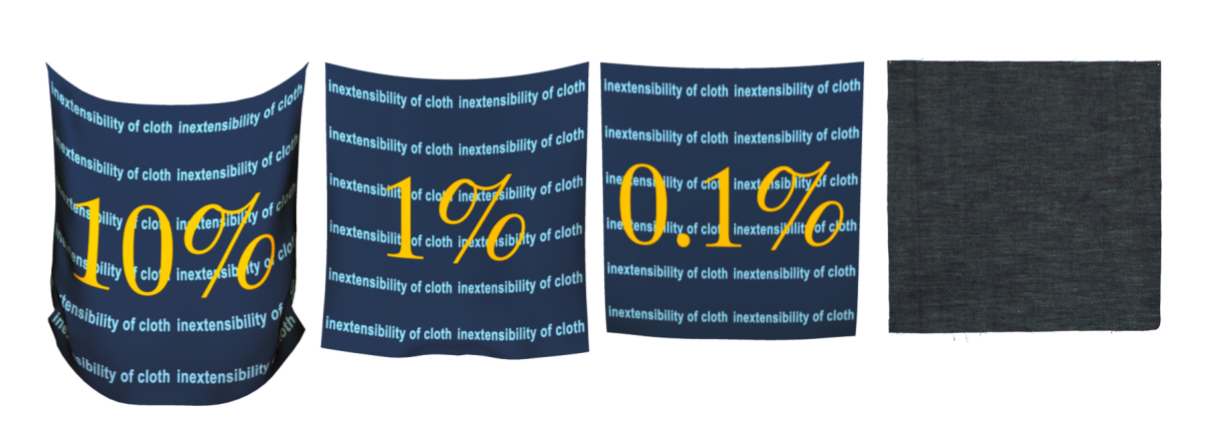
\includegraphics[scale=0.2]{img/inextensible.png}
  \end{figure}
  \item Lagrange function
    \begin{equation*}
      \mathcal{L}(t, \BOLD{x}, \BOLD{\dot x}, \BOLD{\lambda}) = \frac{1}{2}\BOLD{\dot x^T M \dot x} - V(\BOLD{x}) - \sum_i \lambda_i \phi(\BOLD{x})
    \end{equation*}
 \end{itemize}
 %\gridlines 
\end{frame}

\begin{frame}
 \frametitle{Hard Constraints}
 \begin{itemize}
    \item Euler-Lagrange equation
    \begin{equation*}
      \PDIF{\mathcal{L}}{\BOLD{x}}-\frac{d}{dt}\PDIF{\mathcal{L}}{\BOLD{\dot x}} = 0
      \Longrightarrow \BOLD{M\ddot x} = -\PDIF{V}{\BOLD{x}}-\BOLD{J^T\lambda}
    \end{equation*}
    \TikzDraw {
      \visible<2> {
	\node at (-2.5, -1.8) {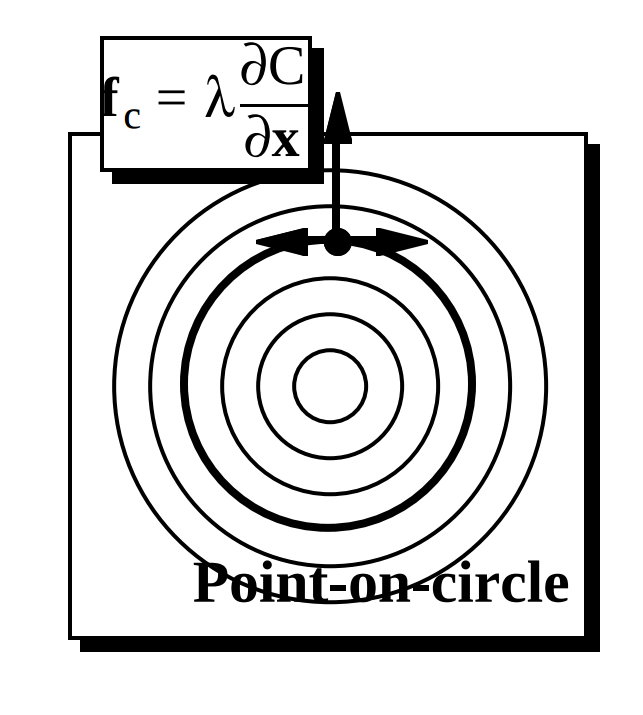
\includegraphics[scale=0.2]{img/cons_force.png}};
	\node at (2.7, -1.8) {\parbox[t]{0.6\textwidth}{
	  \begin{itemize}
	   \item \color{yellow!50}Restrict constraint force to the normal direction.
	   \item Orthogonal to all legal displacements.
	   \item No work, no energy gain or loss.
	  \end{itemize}
	}};
      }
    }
    \pause
    \TikzDraw {
      \visible<2> {
	\draw[red, very thick] (2.3, 1.15) circle (0.6cm);
	\draw[red, very thick] (3.5, 1.15) circle (0.6cm);
	\node at (2, 0.3) { \color{green!50} elastic force};
	\node at (4, 2.0) { \color{green!50} constraint force};
      }
    }
    \pause
    \item Linearization 
    \begin{equation*}
      \begin{pmatrix}
	\BOLD{M}-h^2\BOLD{K} & -\BOLD{J}^T \\
	\BOLD{J} & 0
      \end{pmatrix}
      \begin{pmatrix}
       \BOLD{v}_{+} \\ \BOLD{\mu}_{+}
      \end{pmatrix}
      =
      \begin{pmatrix}
       \BOLD{p}+h\BOLD{f} \\ \BOLD{0}
      \end{pmatrix}
    \end{equation*}
    \TikzDraw {
      \visible<3> {
	\node [fill=DARK!50, draw=black!50, rounded corners=3mm, text opacity=1, fill opacity=0.7] at (0.3, -2.8) {\Large \color{yellow}impulse $\BOLD{\mu}=h\lambda$};
      }
      \visible<4> {
	\draw[red, very thick] (-3, -0.7)--(-3, -2.2)--(0.4, -2.2)--(0.4, -0.7)--(-3, -0.7);
	\node at (-1.2, -2.6) {\huge\color{green!50}  KKT};
      }
    }
 \end{itemize}
 %\gridlines 
 \end{frame}

\begin{frame}
 \frametitle{Compliant Constraints: Regularization}
 \begin{itemize}
  \item constraints$\rightarrow$elasticity
  \begin{equation*}
   V=\frac{1}{2}\BOLD{\phi(x)}^T\BOLD{{\color{orange}{C}}^{-1}\phi(x)}
  \end{equation*}
  \item resulting force
  \begin{equation*}
   \BOLD{f}_c = -\BOLD{J}^T\BOLD{C^{-1}\phi(x)}
  \end{equation*}
  \pause
  \TikzDraw {
    \draw (-0.2, -0.45) node[circle, inner sep=0.15cm, fill=none, draw=red, very thick] (E) {};
    \draw (1.19, -0.45) node[circle, inner sep=0.6cm, fill=none, draw=red, very thick] (F) {};
    \draw (3.5, -1.5) node[circle, inner sep=0.2cm, fill=none, draw=red, very thick] (G) {\Huge \color{green!50} $\lambda$};
    \draw[red, very thick, ->] (E) to [bend right=45] (G);
    \draw[red, very thick, ->] (F) to [bend left=45] (G);
  }
  \pause
  \item dynamic system
  \begin{eqnarray*}
    \BOLD{M\ddot{x}} &=& \BOLD{f}_{ext}+\BOLD{J}^T\BOLD{\lambda} \\
    \BOLD{C\lambda} &=& -\BOLD{\phi}
  \end{eqnarray*}
 \end{itemize}
 %\gridlines
\end{frame}

\begin{frame}
 \frametitle{Compliant Constraints: Regularization}
 \begin{itemize}
  \item Notice
  \begin{equation*}
   \BOLD{C\lambda}_+ = \BOLD{C}\frac{\mu_+}{h}=-\BOLD{\BOLD{\phi}}_+\approx-\BOLD{\phi}-h\BOLD{Jv}_+
  \end{equation*}
  \item Backward integration
    \begin{equation*}
     \begin{pmatrix}
      \BOLD{M} & -\BOLD{J}^T \\
      \BOLD{J} & \frac{1}{h^2}\BOLD{C}
     \end{pmatrix}
     \begin{pmatrix}
      \BOLD{v}_+ \\ \BOLD{\mu}_+
     \end{pmatrix}
     =
     \begin{pmatrix}
      \BOLD{p}+h\BOLD{f}_e \\ -\frac{1}{h}\BOLD{\phi}
     \end{pmatrix}
    \end{equation*}
  \item Schur complement
    \begin{equation*}
      (\BOLD{JM}^{-1}\BOLD{J}^T + \frac{1}{h^2}\BOLD{C})\BOLD{\mu}_+ = -\frac{1}{h}\BOLD{\phi}-\BOLD{JM}^{-1}(\BOLD{p}+h\BOLD{f}_e)
    \end{equation*}
 \end{itemize}
\end{frame}

\begin{frame}
 \frametitle{Compliance Formulation=Penalty?}
 \begin{itemize}
  \item Considering disretization and linearization
    \begin{eqnarray*}
      \BOLD{M}(\BOLD{v}_+-\BOLD{v}) &=& h\BOLD{f}_{e}+h\BOLD{J}^T\BOLD{\lambda}_+ \\
      \BOLD{M}(\BOLD{v}_+-\BOLD{v}) &=& h\BOLD{f}_{e}-h\BOLD{J}^T\BOLD{C}^{-1}\BOLD{\phi}_+ \\
      \BOLD{M}(\BOLD{v}_+-\BOLD{v}) &=& h\BOLD{f}_{e}-h\BOLD{J}^T\BOLD{C}^{-1}(\BOLD{\phi}+h\BOLD{Jv}_+)
    \end{eqnarray*}
  \item System equation 
    \begin{equation*}
      (\BOLD{M}-h^2{\color{red}\BOLD{J}^T\BOLD{C}^{-1}\BOLD{J}})\BOLD{v}_+ = \BOLD{p}+h\BOLD{f}_{e}+h\BOLD{J}^T\BOLD{\lambda}
    \end{equation*}
  \pause
  \TikzDraw {
    \node at (-0.4, -0.4) {\huge \color{red} $\neq \PDIF{\BOLD{f}_c}{\BOLD{x}}$};
  }
  \item Eliminate a part of nonlinearity through \textit{\color{yellow}variable substitution}. WHAT IS IT? HOW IT HELP?
 \end{itemize}
\end{frame}


\begin{frame}
 \frametitle{Compliant Constraints: Summary}
 \begin{itemize}
  \item Loss in part of Jacobian of constraint force.
  \item $\text{stiffness}\rightarrow \infty, \BOLD{K}\rightarrow\text{ill-conditioned}, \BOLD{C}\rightarrow \BOLD{0}$.
  \item Keep the equation numerically tractable, suitable for high stiffness.
  \item $\BOLD{C}$ has a numerical regularization effect.
 \end{itemize}
\end{frame}

\begin{frame}
 \frametitle{Stable Constraints}
 {\color{green}Geometric Stiffness} \& {\color{red}Material Stiffness}
 \begin{figure}[h]
  \centering
  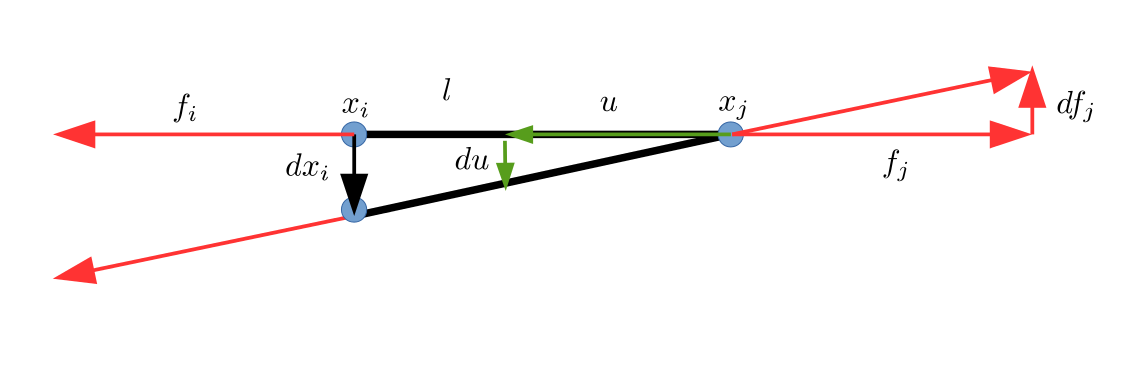
\includegraphics[scale=0.2]{img/geo_stiff.png}
 \end{figure}
 Spring potential: $V=\frac{k}{2}(\bar{l}-l)^2$, $l=\|\BOLD{x}_i-\BOLD{x}_j\|$ 
 \begin{equation*}
  \PDIF{\BOLD{f}_j}{\BOLD{x}_i}=\PDIF{\BOLD{f}_i}{\BOLD{x}_j}=-\PDIF{\BOLD{f}_i}{\BOLD{x}_i}=-\PDIF{\BOLD{f}_j}{\BOLD{x}_j}={\color{red}k\BOLD{uu}^T}\color{green}-\frac{k(\bar l-l)}{l}(\BOLD{I_3}-\BOLD{uu}^T)
 \end{equation*}
\end{frame}

\begin{frame}
 \frametitle{Stiffness Splitting}
 \TikzDraw {
  \node [fill=DARK!50, draw=black!50, rounded corners=3mm, text opacity=1, fill opacity=0.7] at (0, 0) {
    \parbox[t]{0.7\textwidth}{
      \begin{eqnarray*}
	V &=& \frac{1}{2}\BOLD{\phi(x)}^T\BOLD{C}^{-1}\BOLD{\phi(x)} \\
	\BOLD{f} &=& -\PDIF{V}{\BOLD{x}}^T = -\PDIF{\BOLD{\phi}}{\BOLD{x}}^T\PDIF{V}{\BOLD{\phi}}^T = \BOLD{J}^T\BOLD{\lambda} \\
	\BOLD{K} &=& \PDIF{\BOLD{f}}{\BOLD{x}} = {\color{red}\BOLD{J}^T\PDIF{\BOLD{\lambda}}{\BOLD{\phi}}\BOLD{J}}+\color{green}\PDIF{\BOLD{J}}{\BOLD{x}}^T\BOLD{\lambda} \\
	\color{green}\tilde{\BOLD{K}} &\color{green}=& \color{green}\PDIF{\BOLD{J}}{\BOLD{x}}^T\BOLD{\lambda}
      \end{eqnarray*}
    }
  };
 }
\end{frame}

\begin{frame}
 \frametitle{Stiffness Splitting}
  Implicit integration
  \begin{equation*}
   (\BOLD{M}-h^2(\BOLD{J}^T\BOLD{C}^{-1}\BOLD{J}+\tilde{\BOLD{K}}))\BOLD{v}_+=\BOLD{p}+h\BOLD{f}_e-h\BOLD{J}^T\BOLD{\lambda}
  \end{equation*}
  \begin{equation*}
   \color{green}\BOLD{\lambda}_+ = \BOLD{\lambda}+h\BOLD{C}^{-1}\BOLD{Jv}_+
  \end{equation*}
  \begin{equation*}
   \color{red}(\BOLD{M}-h^2\tilde{\BOLD{K}})\BOLD{v}_+ - h\BOLD{J}^T\BOLD{\lambda}_+=\BOLD{p}+h\BOLD{f}_e
  \end{equation*}
  
  
  \begin{equation*}
   \begin{pmatrix}
    \BOLD{M}-h^2\BOLD{\tilde{K}} & -\BOLD{J}^T \\
    \BOLD{J} & \frac{1}{h^2}\BOLD{C}
   \end{pmatrix}
   \begin{pmatrix}
    \BOLD{v}_+ \\ \BOLD{\mu}_+
   \end{pmatrix}
   =
   \begin{pmatrix}
    \BOLD{p}+h\BOLD{f}_e \\ -\frac{1}{h}\BOLD{\phi}
   \end{pmatrix}
  \end{equation*}
  \TikzDraw {
    \draw[->, yellow, very thick] (-2.4, 1.5)--(-2.4, 0.0);
    \draw[yellow, very thick] (-1.8, 0.9)--(-2.4, 0.9);
    \draw[->, yellow, very thick] (2.32, 1.5)--(2.32, -1.8);
    \draw[yellow, very thick] (1.4, -0.5)--(1.4, -1)--(2.32, -1);
  }
  %\gridlines
\end{frame}
  
\begin{frame}
 \frametitle{Stiffness Splitting: Insight}
 \begin{itemize}
  \item {\color{red}Stiffness} vs. {\color{green}Compliance}
  \item {\color{red}Elasticity} vs. {\color{green}Constraints}
  \item Switch between them, to make the matrix well conditioned.
  \item Generalization? Fast mass spring, ARAP, projective dynamics...
 \end{itemize}
\end{frame}


%\begin{frame}
% \frametitle{Conclusion}
% \TikzDraw {
%   \visible<1-> { \node at (-1,1) 
%     {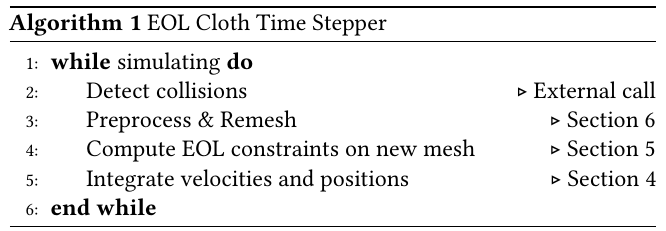
\includegraphics[scale=0.2]{pic/algorithm.png}}; 
%   }
%   \visible<1> {\node at (2,-2) 
%     {\parbox[t]{\textwidth}{\Large$\pi(x_1) = \pi(x_2) = x$}}; 
%   }
%   \visible<1> {\node at (7, -3) 
%     {\parbox[t]{\textwidth}{$\alpha\circ \tau = -\alpha\\ cos(\alpha)=cos(-\alpha)$}};
%   }
% }
% \gridlines
%\end{frame}

\begin{frame}
 \frametitle{Results}
 \begin{figure}
  \centering
  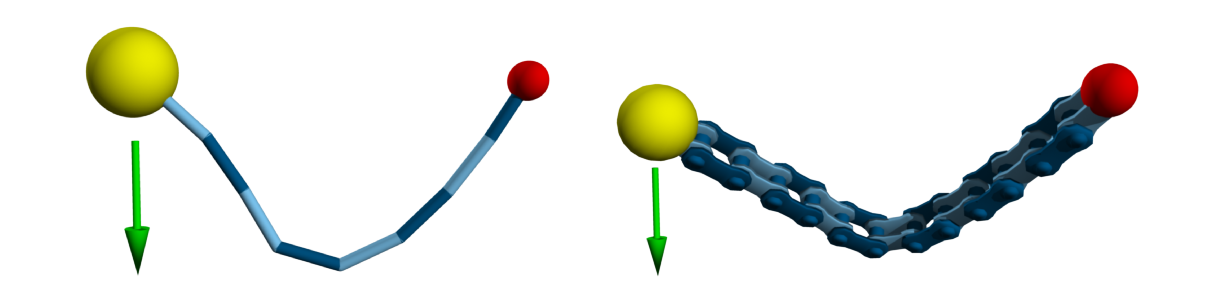
\includegraphics[scale=0.25]{img/cables.png}
 \end{figure}
 \begin{figure}
  \centering
  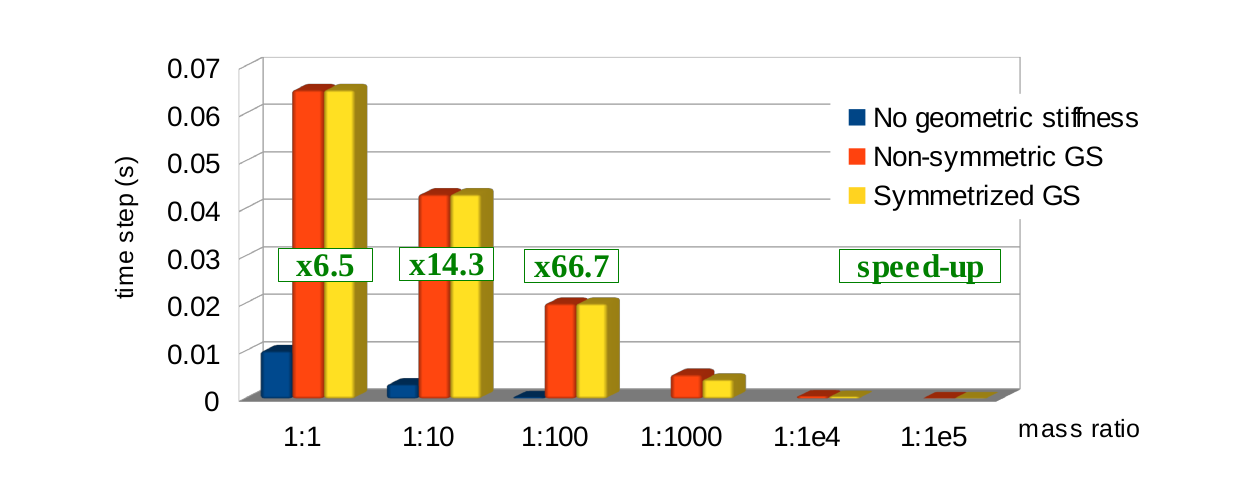
\includegraphics[scale=0.25]{img/statistics.png}
 \end{figure}
\end{frame}

\begin{frame}
 \frametitle{Conclusion}
 \begin{itemize}
  \item Pro: stable and fast convergence even under large time step
  \item Con: a lot of constraints thus bigger system matrix.
  \begin{eqnarray*}
    \text{Green Strain} ~\epsilon&=&\frac{1}{2}(\BOLD{F}^T\BOLD{F}-\BOLD{I})=
    \begin{pmatrix}
     \epsilon_{11} & \epsilon_{12} & \epsilon_{13} \\
     \epsilon_{21} & \epsilon_{22} & \epsilon_{23} \\
     \epsilon_{31} & \epsilon_{32} & \epsilon_{33} \\
    \end{pmatrix} \\
   V &=& \sum_i \frac{1}{2}w_i\epsilon_i^T\BOLD{D}_i\epsilon_i \\
  \end{eqnarray*}
  \item careful observations $\Rightarrow$ good numerical algorithm
 \end{itemize}
 \TikzDraw {
  \draw[->,red, very thick] (2.7,0.62)--(3.1,0.38);
  \draw[->,red, very thick] (3.52, 0.15)--(3.95,-0.10);
  \draw[->,red, very thick] (4.2,-0.10)--(4.2,0.17);
  \draw[->,red, very thick] (4.2,0.38)--(4.2,0.65);
  \draw[->,red, very thick] (3.9,0.78)--(3.6,0.78);
  \node at (0, -1.9) { \color{red} six constraints per tet!};
 }
 %\gridlines
\end{frame}

\begin{frame} 
  \TikzDraw {
    \node at (0, 0.5) {\Huge{Thanks!}};
  }
  %\gridlines
\end{frame}


\end{document}
